\documentclass[aspectratio=169, 10pt]{beamer}
\usepackage[utf8]{inputenc}
\usepackage{amsmath, amssymb, bm, amsfonts}
\usepackage{booktabs}
\usepackage{listings}
\usepackage{graphicx}
\usepackage{tikz}
\usetikzlibrary{arrows.meta, positioning, calc, angles, quotes, shapes.geometric}

% ==============================================================================
% UNIVERSIDAD DE ANTIOQUIA (UdeA) BRANDING & THEME SETUP
% ==============================================================================
\definecolor{UdeAGreen}{HTML}{006241}
\definecolor{UdeAGold}{HTML}{D4AF37}
\definecolor{Charcoal}{HTML}{2B2B2B}
\definecolor{LightBg}{HTML}{F8F9FA}
\definecolor{DarkSlate}{RGB}{15, 23, 42}
\definecolor{AlertRed}{RGB}{220, 38, 38}
\definecolor{SpiceBlue}{RGB}{2, 132, 199}

\setbeamercolor{palette primary}{bg=UdeAGreen, fg=white}
\setbeamercolor{palette secondary}{bg=UdeAGreen, fg=white}
\setbeamercolor{structure}{fg=UdeAGreen}
\setbeamercolor{background canvas}{bg=LightBg}
\setbeamercolor{text}{fg=Charcoal}

% Block Styles
\setbeamercolor{block title}{bg=UdeAGreen, fg=white}
\setbeamercolor{block body}{bg=white, fg=Charcoal}
\setbeamercolor{block title example}{bg=UdeAGold, fg=DarkSlate}
\setbeamercolor{block body example}{bg=white, fg=Charcoal}
\setbeamercolor{block title alerted}{bg=AlertRed, fg=white}
\setbeamercolor{block body alerted}{bg=white, fg=Charcoal}

% --- Custom Header & Footer Setup with Lower-Right Logo (Protected fallback) ---
\setbeamertemplate{headline}{}
\setbeamertemplate{footline}{%
    \leavevmode%
    \hbox{%
        \begin{beamercolorbox}[wd=0.70\paperwidth,ht=2.8ex,dp=1.2ex,leftskip=.3cm]{palette primary}%
            \footnotesize Universidad de Antioquia -- Faculty of Engineering \hfill Module 2: Low-Thrust Trajectories
        \end{beamercolorbox}%
        \begin{beamercolorbox}[wd=0.30\paperwidth,ht=2.8ex,dp=1.2ex,rightskip=.3cm]{palette primary}%
            \hfill \insertframenumber/\inserttotalframenumber\hspace{0.25cm}%
            \IfFileExists{Images/UdeA+simplificado+Negro_Smaller.png}{%
                \raisebox{-0.15ex}{
\includegraphics[height=1.8ex,keepaspectratio]{Images/UdeA+simplificado+Negro_Smaller.png}}%
            }{%
                \textbf{UdeA}%
            }%
        \end{beamercolorbox}%
    }%
    \vskip0pt%
}
\setbeamertemplate{navigation symbols}{}

% Code Listings Configuration
\lstdefinestyle{gmatstyle}{
    backgroundcolor=\color{LightBg},
    basicstyle=\ttfamily\fontsize{5.0pt}{5.8pt}\selectfont\color{Charcoal},
    keywordstyle=\bfseries\color{UdeAGreen},
    commentstyle=\itshape\color{gray},
    stringstyle=\color{UdeAGold!90!black},
    frame=single,
    rulecolor=\color{UdeAGreen},
    breaklines=false,
    showstringspaces=false,
    xleftmargin=2pt,
    xrightmargin=2pt
}

\lstdefinestyle{pythoncode}{
    backgroundcolor=\color{white},
    basicstyle=\ttfamily\fontsize{4.8pt}{5.6pt}\selectfont\color{Charcoal},
    keywordstyle=\bfseries\color{UdeAGreen},
    commentstyle=\itshape\color{gray},
    stringstyle=\color{UdeAGold!90!black},
    numberstyle=\tiny\color{gray},
    numbers=left,
    numbersep=2pt,
    frame=single,
    rulecolor=\color{UdeAGreen!50},
    breaklines=false,
    showstringspaces=false,
    tabsize=2,
    xleftmargin=2pt,
    xrightmargin=2pt
}

\usetheme{Madrid}
\usefonttheme{professionalfonts}

% Positions logo in the upper right corner (Protected fallback)
\logo{%
    \vspace{-0.2cm}\hfill%
    \IfFileExists{Images/UdeA+simplificado+Negro_Smaller.png}{%
        
\includegraphics[width=1cm]{Images/UdeA+simplificado+Negro_Smaller.png}%
    }{}%
    \hspace{0.1cm}%
}

% Metadata & Title Page
\title[Astrodynamics Module 2]{\textbf{Module 3: Low-Thrust Spacecraft Maneuvers}}
\subtitle{Interplanetary Flight Dynamics}
\author{\textbf{Juan Francisco Puerta Ibarra}}
\institute{Aerospace Engineering}
\date{Semester 2026-2}
\titlegraphic{%
    \IfFileExists{Images/UdeA+simplificado+Negro_Smaller.png}{%
        
\includegraphics[width=2.5cm,keepaspectratio]{Images/UdeA+simplificado+Negro_Smaller.png}%
    }{}%
}

\begin{document}

% ==============================================================================
% TITLE SLIDE
% ==============================================================================
\begin{frame}[plain]
    \titlepage
    \begin{center}
        \scriptsize \textcolor{DarkSlate}{\textit{Analytical Flight Mechanics, Numerical Propagation, and GMAT Targeting}}
    \end{center}
\end{frame}

% --- SLIDE 3.1: IMPULSIVE VS. FINITE REALITY ---
\begin{frame}{Continuous Thrust Trajectories: The Paradigm Shift}
    \begin{columns}[T]
        \begin{column}{0.49\textwidth}
            \begin{block}{The Classical Impulsive Model}
                \scriptsize
                \begin{itemize}\setlength{\itemsep}{2pt}\setlength{\topsep}{1pt}
                    \item \textbf{Infinitesimal Burn Duration:} Assumes burn time $\Delta t \to 0$.
                    \item \textbf{Invariant Position:} Spacecraft position $\mathbf{r}$ remains frozen during velocity change.
                    \item \textbf{Instantaneous Vector Jump:} $\mathbf{v}^+ = \mathbf{v}^- + \Delta \mathbf{v}$.
                    \item Localized to optimal apsidal points (e.g., periapsis Oberth burns).
                \end{itemize}
            \end{block}
            \vspace{-0.1cm}
            \begin{alertblock}{The Operational Reality: Finite Maneuvers}
                \scriptsize
                \begin{itemize}\setlength{\itemsep}{2pt}\setlength{\topsep}{1pt}
                    \item Chemical engines burn for minutes; Solar Electric Propulsion (SEP) thrusters burn for weeks or months.
                    \item Spacecraft position $\mathbf{r}(t)$ changes significantly during the burn arc.
                    \item Acceleration is sub-Newtonian ($10^{-3}$ to $10^{-6}$ g), requiring continuous integration over many revolutions.
                \end{itemize}
            \end{alertblock}
        \end{column}

        \begin{column}{0.49\textwidth}
            \begin{block}{The Fundamental Trade-Off: Mass vs. Time}
                \scriptsize
                \begin{itemize}\setlength{\itemsep}{2pt}\setlength{\topsep}{1pt}
                    \item \textbf{Gravity Loss Penalty:} Thrusting away from apsides requires higher cumulative velocity increment ($\Delta V_{\text{spiral}} > \Delta V_{\text{Hohmann}}$).
                    \item \textbf{Specific Impulse Leverage:} Electric thrusters achieve $I_{\text{sp}} \sim 3{,}000\text{--}5{,}000\text{ s}$ ($\sim 10\times$ chemical rockets).
                    \item \textbf{Tsiolkovsky Exponential Advantage:}
                    $$\frac{m_f}{m_0} = \exp\left(-\frac{\Delta V}{I_{\text{sp}} g_0}\right)$$
                    \item Drastically reduces propellant mass fraction, liberating mass for science payload.
                \end{itemize}
            \end{block}
            \centering
            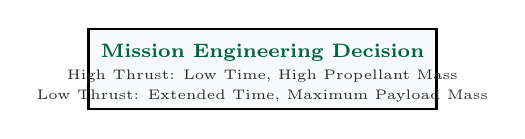
\begin{tikzpicture}[scale=0.85]
                \draw[thick, fill=LightBg] (0,0) rectangle (5.2,1.2);
                \node[font=\scriptsize\bfseries, color=UdeAGreen] at (2.6, 0.85) {Mission Engineering Decision};
                \node[font=\tiny, Charcoal] at (2.6, 0.50) {High Thrust: Low Time, High Propellant Mass};
                \node[font=\tiny, Charcoal] at (2.6, 0.20) {Low Thrust: Extended Time, Maximum Payload Mass};
            \end{tikzpicture}
        \end{column}
    \end{columns}
\end{frame}

% ------------------------------------------------------------------------------
% SLIDE 3.1: IMPULSIVE VS. LOW-THRUST COMPARISON MATRIX
% ------------------------------------------------------------------------------
% ------------------------------------------------------------------------------
% SLIDE 3.1: IMPULSIVE VS. LOW-THRUST COMPARISON MATRIX
% ------------------------------------------------------------------------------
% ------------------------------------------------------------------------------
% SLIDE 3.1: IMPULSIVE VS. LOW-THRUST COMPARISON MATRIX
% ------------------------------------------------------------------------------
\begin{frame}{Maneuver Architectures: Impulsive vs. Continuous Low-Thrust}
    \begin{columns}[T]
        \begin{column}{0.48\textwidth}
            \begin{block}{The Physical Analogy}
                \scriptsize
                \begin{itemize}\setlength{\itemsep}{1.2pt}\setlength{\topsep}{0pt}
                    \item \textbf{Impulsive (The Cannon):} Energy is injected instantly at discrete points; vehicle coasts along unperturbed Keplerian conics.
                    \item \textbf{Continuous (The Ramp):} A persistent whisper of thrust (mN to N) slowly unwinds or reshapes the orbit over weeks or months.
                \end{itemize}
            \end{block}
            \vspace{-0.15cm}
            \begin{alertblock}{The Core Mission Trade-Off}
                \scriptsize
                We trade \textbf{Time for Mass}:
                \begin{itemize}\setlength{\itemsep}{1pt}\setlength{\topsep}{0pt}
                    \item Continuous thrust incurs high gravity losses ($\Delta V_{\text{spiral}} > \Delta V_{\text{Hohmann}}$).
                    \item However, electric systems achieve $I_{\text{sp}} > 3{,}000\text{ s}$ ($10\times$ chemical), drastically reducing propellant fraction.
                \end{itemize}
            \end{alertblock}
        \end{column}

        \begin{column}{0.50\textwidth}
            \begin{block}{Architectural Comparison Matrix}
                \scriptsize
                \centering
                \renewcommand{\arraystretch}{1.1}
                \begin{tabular}{lcc}
                    \toprule
                    \textbf{Metric} & \textbf{Impulsive} & \textbf{Low-Thrust} \\
                    \midrule
                    Propulsion & Chemical & Electric / SEP \\
                    Thrust ($T$) & $10^2 - 10^6\text{ N}$ & $10^{-3} - 10^0\text{ N}$ \\
                    $I_{\text{sp}}$ & $300 - 450\text{ s}$ & $1{,}500 - 5{,}000\text{ s}$ \\
                    Burn Time & Seconds to min & Weeks to months \\
                    Path Geometry & Conic + Coast & Continuous Spiral \\
                    Gravity Loss & Minimal (Oberth) & Substantial \\
                    Dry Payload & Bounded by fuel & Maximized \\
                    \bottomrule
                \end{tabular}
            \end{block}
        \end{column}
    \end{columns}
\end{frame}

% ------------------------------------------------------------------------------
% SLIDE 3.2: MATHEMATICAL FORMULATION & STATE-SPACE DIVERGENCE
% ------------------------------------------------------------------------------
\begin{frame}{Dynamic Formulation: Conic Jumps vs. 7D State Integration}
    \begin{columns}[T]
        \begin{column}{0.48\textwidth}
            \begin{block}{Impulsive Formulation ($\mathbb{R}^6$ Conic Jumps)}
                \scriptsize
                Maneuvers are modeled as point velocity discontinuities:
                \par\vspace{1pt}
                {\centering $\mathbf{r}^+ = \mathbf{r}^-, \quad \mathbf{v}^+ = \mathbf{v}^- + \Delta \mathbf{v}$ \par}
                \begin{itemize}\setlength{\itemsep}{1.2pt}\setlength{\topsep}{0pt}
                    \item \textbf{Position Invariance:} $\Delta t \to 0$ assumes orbital position is frozen during firing.
                    \item \textbf{Decoupled Mass Step:} Mass is subtracted discretely via the Tsiolkovsky equation after each burn:
                    \par\vspace{1pt}
                    {\centering $\Delta m = m_0 \left[1 - \exp\left(-\frac{\Delta v}{I_{\text{sp}} g_0}\right)\right]$ \par}
                    \item Propagator takes massive steps during unpowered coast arcs.
                \end{itemize}
            \end{block}
        \end{column}

        \begin{column}{0.48\textwidth}
            \begin{exampleblock}{Continuous Low-Thrust Dynamics ($\mathbb{R}^7$ EOM)}
                \scriptsize
                Position changes significantly while thrusting; mass becomes a dynamic coordinate:
                \par\vspace{1pt}
                {\centering $\mathbf{Y}(t) = [\mathbf{r}^T, \; \mathbf{v}^T, \; m]^T \in \mathbb{R}^7$ \par}
                \vspace{-2pt}
                \begin{equation*}
                    \frac{d\mathbf{Y}}{dt} = \begin{bmatrix} 
                        \mathbf{v} \\ 
                        -\frac{\mu}{r^3}\mathbf{r} + \frac{\mathbf{T}(t)}{m(t)} + \mathbf{a}_{\text{pert}} \\ 
                        -\frac{\|\mathbf{T}(t)\|}{I_{\text{sp}} g_0} 
                    \end{bmatrix}
                \end{equation*}
                \begin{itemize}\setlength{\itemsep}{1.2pt}\setlength{\topsep}{0pt}
                    \item \textbf{Acceleration Coupling:} Constant $T$ causes acceleration $a(t) = T/m(t)$ to rise continuously.
                    \item \textbf{Adaptive Step Reduction:} Numerical engines must shrink step sizes across thousands of revolutions.
                \end{itemize}
            \end{exampleblock}
        \end{column}
    \end{columns}
\end{frame}

% ------------------------------------------------------------------------------
% SLIDE 3.3: MISSION DESIGN TOOLCHAIN DIVERGENCE
% ------------------------------------------------------------------------------
\begin{frame}{Flight Mechanics Toolchain: Targeters vs. Optimizers}
    \begin{columns}[T]
        \begin{column}{0.48\textwidth}
            \begin{block}{Impulsive Mission Workflow}
                \scriptsize
                \begin{itemize}\setlength{\itemsep}{1.5pt}\setlength{\topsep}{0pt}
                    \item \textbf{Boundary Value Engine:} Lambert's problem connects departure and arrival positions over fixed transfer times.
                    \item \textbf{Porkchop Map Exploration:} Fast scans over launch and arrival windows calculate $C_3$ and $\Delta V$ contours.
                    \item \textbf{Differential Correctors:} Local Newton-Raphson shooting methods iteratively converge on target B-plane coordinates.
                \end{itemize}
            \end{block}
            \vspace{-0.15cm}
            \begin{alertblock}{Why Simple Targeters Fail in Low-Thrust}
                \scriptsize
                \begin{itemize}\setlength{\itemsep}{1.2pt}\setlength{\topsep}{0pt}
                    \item Continuous burns span hundreds to thousands of orbits.
                    \item Sensitivities become highly cyclical and non-linear, causing differential correctors to easily diverge or encounter singular Jacobians.
                \end{itemize}
            \end{alertblock}
        \end{column}

        \begin{column}{0.48\textwidth}
            \begin{exampleblock}{Low-Thrust Mission Workflow}
                \scriptsize
                \begin{itemize}\setlength{\itemsep}{1.5pt}\setlength{\topsep}{0pt}
                    \item \textbf{Continuous Steering Laws:} Solves for a continuous thrust orientation vector history $\hat{\mathbf{u}}(t)$.
                    \item \textbf{Pontryagin's Minimum Principle (PMP):} Formulates the Hamiltonian $\mathcal{H}$ with costate tracking:
                    \par\vspace{1pt}
                    {\centering $\hat{\mathbf{u}}^*(t) = -\frac{\boldsymbol{\lambda}_v}{\|\boldsymbol{\lambda}_v\|} \quad (\text{Primer Vector Steering})$ \par}
                    \item \textbf{Nonlinear Programming (NLP):} Deploys direct collocation or optimizers (e.g., SNOPT, IPOPT) to minimize propellant under path constraints.
                \end{itemize}
            \end{exampleblock}
        \end{column}
    \end{columns}
\end{frame}

% --- SLIDE 3.2: 7D STATE EXPANSION ---
\begin{frame}{Finite Maneuvers: Dynamic Equations and 7D State Vector}
    \begin{columns}[T]
        \begin{column}{0.54\textwidth}
            \begin{block}{Translational Dynamics \& Mass Depletion}
                \scriptsize
                Under finite thrust, vehicle mass depletes continuously as propellant is expelled, coupling vehicle acceleration directly to time:
                \begin{equation}
                    \ddot{\mathbf{r}} = -\frac{\mu}{r^3}\mathbf{r} + \mathbf{a}_{\text{perturbations}} + \frac{\mathbf{T}}{m(t)}
                \end{equation}
                \begin{equation}
                    \dot{m}(t) = -\frac{\|\mathbf{T}\|}{I_{\text{sp}} g_0}
                \end{equation}
                \begin{itemize}\setlength{\itemsep}{1.5pt}
                    \item $\mathbf{T}$ is the thrust vector; $g_0 = 9.80665\text{ m/s}^2$.
                    \item Because $m(t)$ is in the denominator, constant thrust magnitude $\|\mathbf{T}\|$ produces continuously increasing acceleration over time.
                \end{itemize}
            \end{block}
        \end{column}

        \begin{column}{0.44\textwidth}
            \begin{exampleblock}{State-Space Expansion ($\mathbb{R}^6 \to \mathbb{R}^7$)}
                \scriptsize
                In Keplerian dynamics, the state vector is 6D ($\mathbf{r}, \mathbf{v}$). Continuous finite burns require expanding the state vector to include mass as a dynamic coordinate:
                \begin{equation}
                    \mathbf{Y}(t) = \begin{bmatrix} \mathbf{r}(t) \\ \mathbf{v}(t) \\ m(t) \end{bmatrix} = \begin{bmatrix} x \\ y \\ z \\ v_x \\ v_y \\ v_z \\ m \end{bmatrix} \in \mathbb{R}^7
                \end{equation}
                The first-order derivative integrated by numerical solvers is:
                \begin{equation}
                    \frac{d\mathbf{Y}}{dt} = \begin{bmatrix} \mathbf{v} \\ \mathbf{a}_{\text{grav}} + \mathbf{a}_{\text{thrust}} + \mathbf{a}_{\text{pert}} \\ -\|\mathbf{T}\| / (I_{\text{sp}} g_0) \end{bmatrix}
                \end{equation}
            \end{exampleblock}
        \end{column}
    \end{columns}
\end{frame}

% --- SLIDE 3.3: QUASI-CIRCULAR SPIRAL ---
\begin{frame}{The Quasi-Circular Spiral and Gravity Losses}
    \begin{columns}[T]
        \begin{column}{0.54\textwidth}
            \begin{block}{The Quasi-Circular Outward Spiral}
                \scriptsize
                \begin{itemize}\setlength{\itemsep}{2pt}\setlength{\topsep}{1pt}
                    \item For micro-thrust acceleration ($a_{\text{thrust}} < 10^{-4}\text{ g}$), the orbit does not become highly eccentric; it slowly spirals outward through continuous tangential acceleration.
                    \item \textbf{Vallado Analytical Approximation (Section 6.7):} Transferring between circular radii $r_1$ and $r_2$ requires:
                    $$\Delta V_{\text{spiral}} \approx |v_{c1} - v_{c2}| = \left|\sqrt{\frac{\mu}{r_1}} - \sqrt{\frac{\mu}{r_2}}\right|$$
                    \item Equal to the absolute difference between circular speeds.
                \end{itemize}
            \end{block}
            \vspace{-0.1cm}
            \begin{alertblock}{Gravity Loss Quantification}
                \scriptsize
                \begin{itemize}\setlength{\itemsep}{1.5pt}
                    \item Hohmann transfers concentrate burns strictly at apsides, maximizing orbital energy changes.
                    \item Continuous spirals fire across the entire orbit, incurring substantial gravity losses: $\Delta V_{\text{spiral}} > \Delta V_{\text{Hohmann}}$.
                \end{itemize}
            \end{alertblock}
        \end{column}

        \begin{column}{0.44\textwidth}
            \centering
            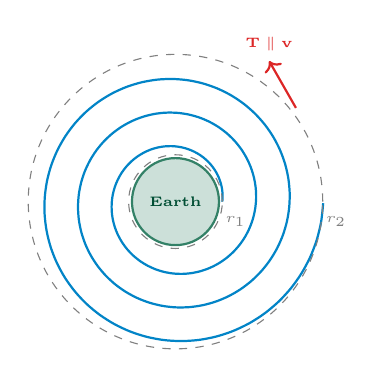
\begin{tikzpicture}[scale=0.85]
                \filldraw[color=UdeAGreen!80, fill=UdeAGreen!20, thick] (0,0) circle (0.65cm);
                \node[font=\tiny\bfseries, color=UdeAGreen!80!black] at (0,0) {Earth};
                
                \draw[domain=0:18.84, variable=\t, samples=150, smooth, thick, color=SpiceBlue]
                    plot ({(0.70 + 0.08*\t)*cos(deg(\t))}, {(0.70 + 0.08*\t)*sin(deg(\t))});
                    
                \draw[thick, ->, color=AlertRed] (1.8, 1.4) -- (1.4, 2.1) node[above, font=\tiny\bfseries] {$\mathbf{T} \parallel \mathbf{v}$};
                \draw[dashed, color=gray] (0,0) circle (0.70cm);
                \node[font=\tiny, color=gray] at (0.9, -0.3) {$r_1$};
                \draw[dashed, color=gray] (0,0) circle (2.20cm);
                \node[font=\tiny, color=gray] at (2.4, -0.3) {$r_2$};
            \end{tikzpicture}
            \par\smallskip
            \scriptsize \textcolor{Charcoal}{\textit{Continuous tangential thrusting spirals outward over hundreds of revolutions.}}
        \end{column}
    \end{columns}
\end{frame}

% --- SLIDE 3.4: EDELBAUM STEERING ---
% --- SLIDE: EDELBAUM'S OPTIMAL STEERING (ZERO OVERFLOW) ---
\begin{frame}{Non-Coplanar Transfers: Edelbaum's Optimal Steering}
    \begin{columns}[T]
        % --- Left Column: Mechanics & Continuous Penalty ---
        \begin{column}{0.53\textwidth}
            \begin{block}{Simultaneous Altitude Raise and Inclination Change}
                \scriptsize
                \begin{itemize}\setlength{\itemsep}{1.2pt}\setlength{\topsep}{0pt}
                    \item Sequential maneuvers (spiraling out, then executing nodal burns) are severely inefficient for electric propulsion.
                    \item \textbf{Edelbaum (1961):} Closed-form analytical $\Delta V$ for simultaneous continuous transfer between circular orbits:
                    \par\vspace{1.5pt}
                    {\centering $\displaystyle \Delta V = \sqrt{v_1^2 + v_2^2 - 2v_1 v_2 \cos\left(\frac{\pi}{2}\Delta i\right)}$ \par}
                    \vspace{1.5pt}
                    \item $v_1, v_2$: Circular velocities; $\Delta i$: plane change in radians.
                \end{itemize}
            \end{block}

            \vspace{-0.22cm}

            \begin{block}{The Continuous Thrust Penalty Factor ($\pi/2$)}
                \scriptsize
                \begin{itemize}\setlength{\itemsep}{1.2pt}\setlength{\topsep}{0pt}
                    \item Impulsive burns change inclination at nodes with $100\%$ geometric efficiency.
                    \item Continuous thrust fires over entire orbits; at $90^\circ$ from nodes, normal thrust produces zero plane change.
                    \item Orbit-averaged efficiency is $2/\pi$, yielding the $\Delta V$ penalty factor $\frac{\pi}{2} \approx 1.57$ inside the cosine argument.
                \end{itemize}
            \end{block}
        \end{column}

        % --- Right Column: Yaw Synergy & Vector Geometry ---
        \begin{column}{0.45\textwidth}
            \begin{alertblock}{The Synergy of Yaw Steering}
                \scriptsize
                \begin{itemize}\setlength{\itemsep}{1.2pt}\setlength{\topsep}{0pt}
                    \item Tilting thrust out-of-plane by yaw angle $\beta$ yields normal acceleration while retaining tangential drive.
                    \item \textbf{Small Angle Power:} Tilting by $\beta = 5^\circ$ yields out-of-plane force while preserving:
                    \par\vspace{1pt}
                    {\centering $\cos(5^\circ) = 0.996 \implies 99.6\%\text{ forward thrust}$ \par}
                \end{itemize}
            \end{alertblock}

            \vspace{-0.05cm}
            \centering
            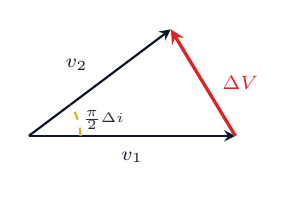
\begin{tikzpicture}[scale=0.82, >=stealth]
                % Base v1
                \draw[thick, ->, color=DarkSlate] (0,0) -- (3.2,0) node[midway, below=2pt, font=\scriptsize] {$v_1$};
                % Vector v2
                \draw[thick, ->, color=DarkSlate] (0,0) -- (2.2, 1.65) node[midway, above left=1pt, font=\scriptsize] {$v_2$};
                % Delta V Vector
                \draw[very thick, ->, color=AlertRed] (3.2,0) -- (2.2, 1.65) node[midway, right=3pt, font=\scriptsize\bfseries] {$\Delta V$};
                % Angle Arc
                \draw[dashed, color=UdeAGold, thick] (0.8,0) arc (0:37:0.8);
                \node[font=\tiny, color=Charcoal] at (1.15,0.24) {$\frac{\pi}{2}\Delta i$};
            \end{tikzpicture}
            \par\vspace{1pt}
            \scriptsize \textcolor{Charcoal}{\textit{Geometric equivalence to the Law of Cosines.}}
        \end{column}
    \end{columns}
\end{frame}

\begin{frame}{Low-Thrust Concepts and Definitions}
    \begin{figure}
        \centering
        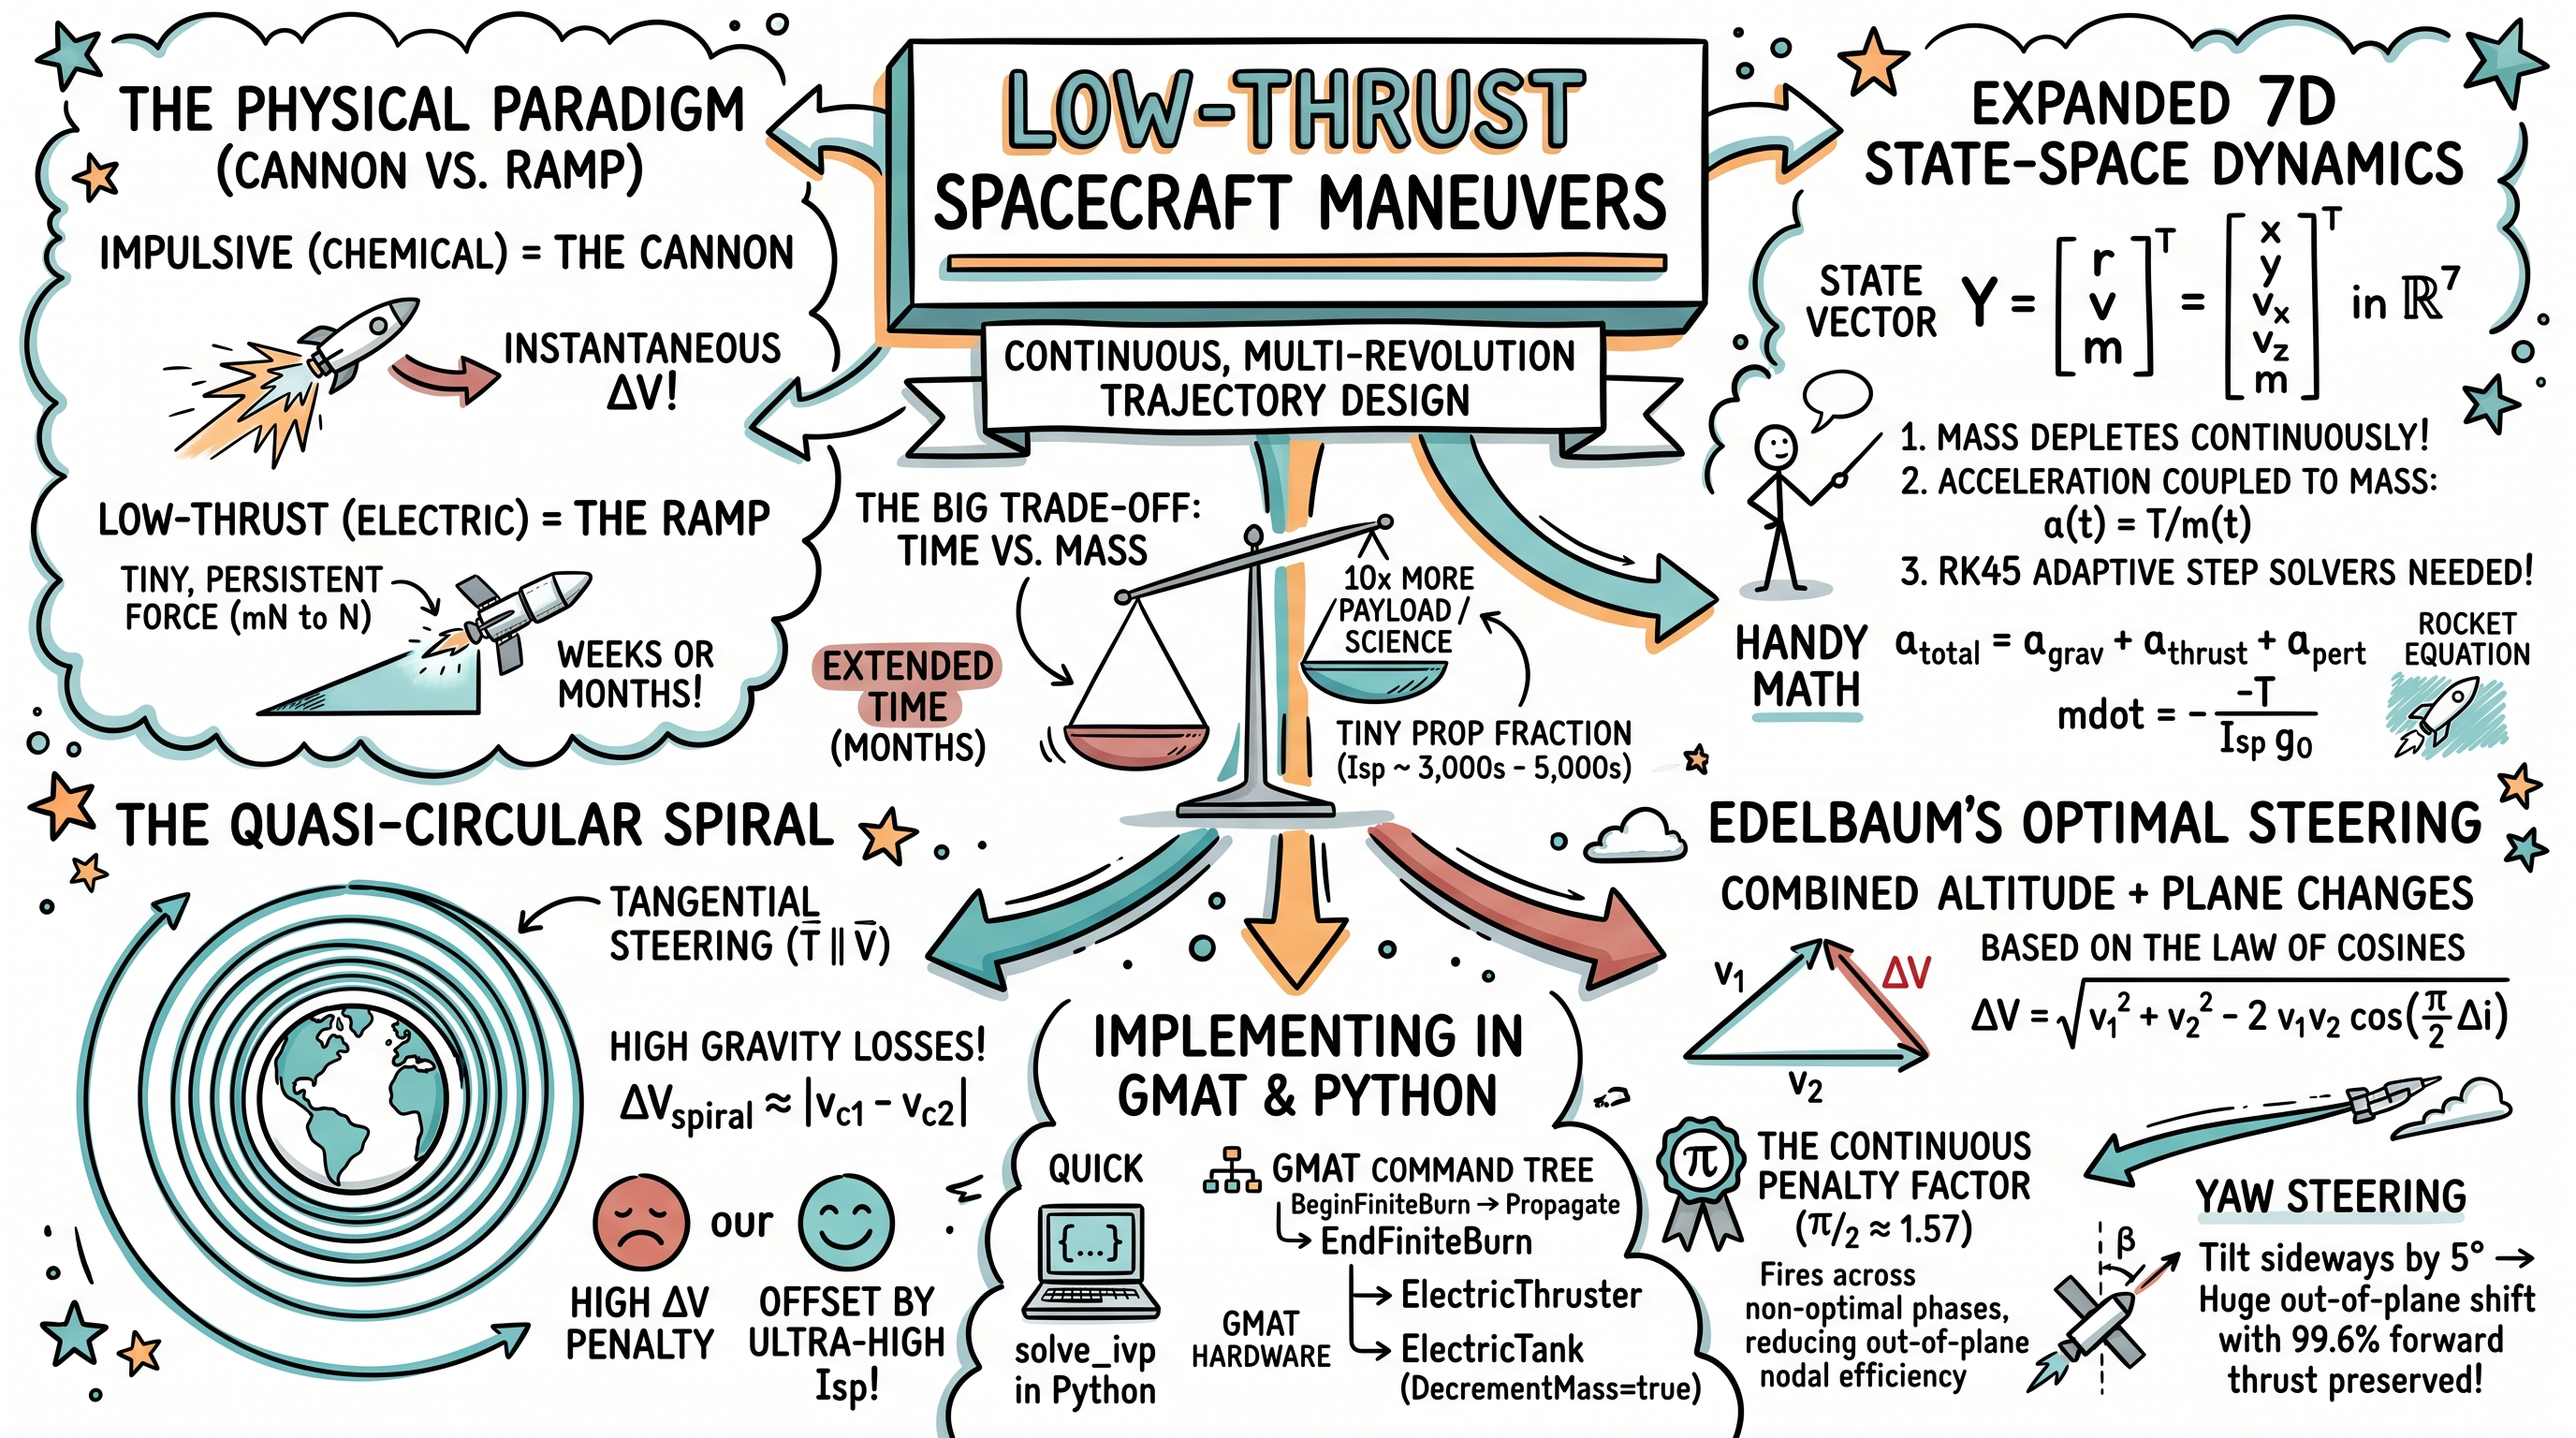
\includegraphics[width=0.80\textwidth]{Images/LT_1.png}
    \end{figure}
\end{frame}

% --- SLIDE 3.5: PYTHON IMPLEMENTATION ---
\begin{frame}[fragile]{Numerical Trajectory Propagation: Python Derivative Engine}
    \begin{columns}[T]
        \begin{column}{0.49\textwidth}
            \begin{block}{Algorithmic Formulation}
                \scriptsize
                \begin{enumerate}\setlength{\itemsep}{1.5pt}\setlength{\topsep}{1pt}
                    \item Unpack $\mathbf{Y} \in \mathbb{R}^7$: position $\mathbf{r}$, velocity $\mathbf{v}$, and mass $m$.
                    \item Compute central gravity acceleration: $\mathbf{a}_{\text{grav}} = -\frac{\mu}{\|\mathbf{r}\|^3}\mathbf{r}$.
                    \item Form unit tangent vector $\hat{\mathbf{u}}_v = \mathbf{v}/\|\mathbf{v}\|$.
                    \item Compute thrust acceleration: $\mathbf{a}_{\text{thrust}} = \frac{T}{m} \hat{\mathbf{u}}_v$.
                    \item Mass depletion: $\dot{m} = -T / (I_{\text{sp}} g_0)$.
                    \item Concatenate derivative vector: $d\mathbf{Y}/dt = [\mathbf{v},\, \mathbf{a}_{\text{total}},\, \dot{m}]^T$.
                \end{enumerate}
            \end{block}
            \vspace{-0.1cm}
            \begin{alertblock}{Solver Selection}
                \scriptsize
                Propagated via adaptive Runge-Kutta solvers (e.g., SciPy's \texttt{DOP853} or \texttt{RK45}).
            \end{alertblock}
        \end{column}

        \begin{column}{0.49\textwidth}
\begin{lstlisting}[style=pythoncode]
import numpy as np
from scipy.integrate import solve_ivp

def low_thrust_ode(t, state, mu, thrust, isp, g0):
    # 1. Unpack 7D State Vector
    r_vec = state[0:3]
    v_vec = state[3:6]
    m     = state[6]
    
    # 2. Central Body Gravity Acceleration
    r_mag  = np.linalg.norm(r_vec)
    a_grav = (-mu / r_mag**3) * r_vec
    
    # 3. Tangential Steering Unit Vector
    v_mag    = np.linalg.norm(v_vec)
    u_v      = v_vec / v_mag
    a_thrust = (thrust / m) * u_v
    
    # 4. Total Acceleration & Mass Depletion
    a_total = a_grav + a_thrust
    mdot    = -thrust / (isp * g0)
    
    # 5. Return 7D Derivative Array
    return np.concatenate((v_vec, a_total, [mdot]))

# Execution: solve_ivp(low_thrust_ode, [0, t_final], y0, 
#                      args=(mu, T, Isp, g0), rtol=1e-10)
\end{lstlisting}
        \end{column}
    \end{columns}
\end{frame}

% --- SLIDE 3.6: GMAT SCRIPTING ---
\begin{frame}[fragile]{Finite Burn Modeling in NASA GMAT}
    \begin{columns}[T]
        \begin{column}{0.49\textwidth}
            \begin{block}{Physical Hardware vs. Impulsive Deltas}
                \scriptsize
                \begin{itemize}\setlength{\itemsep}{2pt}\setlength{\topsep}{1pt}
                    \item Finite maneuvers require abandoning instantaneous \texttt{ImpulsiveBurn} objects to configure real spacecraft subsystems.
                    \item Must instantiate an \texttt{ElectricThruster} and attach it to an \texttt{ElectricTank} resource.
                    \item Thruster requires explicit operational parameters: $I_{\text{sp}}$, thrust magnitude, and \texttt{DecrementMass = true}.
                \end{itemize}
            \end{block}
            \vspace{-0.1cm}
            \begin{alertblock}{Optimizers vs. Targeters}
                \scriptsize
                \begin{itemize}\setlength{\itemsep}{1.5pt}
                    \item Standard Differential Correctors (DC) often diverge or exceed iteration limits over multi-revolution transfers.
                    \item Mission design uses \textbf{Nonlinear Optimizers} (e.g., VF13ad, SNOPT) to minimize burn duration under orbital boundary constraints.
                \end{itemize}
            \end{alertblock}
        \end{column}

        \begin{column}{0.49\textwidth}
\begin{lstlisting}[style=gmatstyle]
% ==========================================
% 1. Spacecraft Hardware Configuration
% ==========================================
Create ElectricThruster IonEngine;
IonEngine.CoordinateSystem = Local;
IonEngine.Origin           = Earth;
IonEngine.Axes             = VNB;
IonEngine.Thrust1          = 0.5;   % Thrust in Newtons
IonEngine.Isp              = 3000;  % Specific Impulse (s)
IonEngine.DecrementMass    = true;

Create ElectricTank XenonTank;
XenonTank.FuelMass         = 50.0;  % Propellant Mass (kg)

SC.Thrusters               = {IonEngine};
SC.Tanks                   = {XenonTank};

% ==========================================
% 2. Mission Sequence: Finite Maneuver Loop
% ==========================================
BeginMissionSequence;

% Activate continuous low-thrust arc
BeginFiniteBurn IonEngine(SC);

% Numerically propagate until target SMA is reached
Propagate EarthProp(SC) {SC.Earth.SMA = 42164};

% Terminate finite burn
EndFiniteBurn IonEngine(SC);
\end{lstlisting}
        \end{column}
    \end{columns}
\end{frame}

% --- SLIDE 3.7: LAB VALIDATION BENCHMARK ---
\begin{frame}{Validation Benchmark: Active Debris Removal (12U CubeSat)}
    \begin{columns}[T]
        \begin{column}{0.54\textwidth}
            \begin{block}{Mission Architecture Comparison}
                \scriptsize
                \textbf{Scenario:} A 12U CubeSat deploys at $400\text{ km}$ LEO and must rendezvous with debris at $600\text{ km}$ with an orbital inclination offset $\Delta i = 2^\circ$.
                \vspace{0.1cm}
                \begin{itemize}\setlength{\itemsep}{2pt}
                    \item \textbf{Impulsive (Green Monopropellant):} $I_{\text{sp}} = 220\text{ s}$. Performs two Hohmann burns to raise altitude, then a pure plane-change impulse at the line of nodes.
                    \item \textbf{Low-Thrust (Micro-Ion Thruster):} $I_{\text{sp}} = 1{,}500\text{ s}$, $T = 2\text{ mN}$. Continuous outward spiral combined with simultaneous yaw steering.
                \end{itemize}
            \end{block}
            \vspace{-0.1cm}
            \begin{exampleblock}{Validation Protocol}
                \scriptsize
                Propagate the low-thrust transfer for 30 days in both environments. Cross-validate final Semi-Major Axis ($a$) and final vehicle mass ($m$) between SciPy and GMAT to verify the 7D integration physics.
            \end{exampleblock}
        \end{column}

        \begin{column}{0.44\textwidth}
            \begin{block}{Summary Benchmark Metrics}
                \scriptsize
                \centering
                \begin{tabular}{lcc}
                    \toprule
                    \textbf{Parameter} & \textbf{Impulsive} & \textbf{Low-Thrust} \\
                    \midrule
                    Propulsion & Monoprop & Micro-Ion \\
                    $I_{\text{sp}}$ & $220\text{ s}$ & $1{,}500\text{ s}$ \\
                    Thrust & $> 1\text{ N}$ & $2\text{ mN}$ \\
                    Transfer Time & Hours & Weeks \\
                    Fuel Mass Fraction & Large & Minimal \\
                    Steering & Node-locked & Edelbaum Yaw \\
                    \bottomrule
                \end{tabular}
            \end{block}
            \vspace{0.1cm}
            \begin{alertblock}{Validation Criterion}
                \scriptsize
                $$\|a_{\text{Python}} - a_{\text{GMAT}}\| < \epsilon_a, \quad \|m_{\text{Python}} - m_{\text{GMAT}}\| < \epsilon_m$$
            \end{alertblock}
        \end{column}
    \end{columns}
\end{frame}

\end{document}